% Options for packages loaded elsewhere
\PassOptionsToPackage{unicode}{hyperref}
\PassOptionsToPackage{hyphens}{url}
\PassOptionsToPackage{dvipsnames,svgnames,x11names}{xcolor}
%
\documentclass[
  12pt,
  a4paper,
  DIV=11,
  numbers=noendperiod,
  twoside,
  open=any]{scrartcl}

\usepackage{amsmath,amssymb}
\usepackage{iftex}
\ifPDFTeX
  \usepackage[T1]{fontenc}
  \usepackage[utf8]{inputenc}
  \usepackage{textcomp} % provide euro and other symbols
\else % if luatex or xetex
  \usepackage{unicode-math}
  \defaultfontfeatures{Scale=MatchLowercase}
  \defaultfontfeatures[\rmfamily]{Ligatures=TeX,Scale=1}
\fi
\usepackage{lmodern}
\ifPDFTeX\else  
    % xetex/luatex font selection
  \setmainfont[]{Minion Pro}
  \setsansfont[]{Minion Pro}
  \setmonofont[]{Menlo}
  \setmathfont[]{KpMath-Regular}
\fi
% Use upquote if available, for straight quotes in verbatim environments
\IfFileExists{upquote.sty}{\usepackage{upquote}}{}
\IfFileExists{microtype.sty}{% use microtype if available
  \usepackage[]{microtype}
  \UseMicrotypeSet[protrusion]{basicmath} % disable protrusion for tt fonts
}{}
\makeatletter
\@ifundefined{KOMAClassName}{% if non-KOMA class
  \IfFileExists{parskip.sty}{%
    \usepackage{parskip}
  }{% else
    \setlength{\parindent}{0pt}
    \setlength{\parskip}{6pt plus 2pt minus 1pt}}
}{% if KOMA class
  \KOMAoptions{parskip=half}}
\makeatother
\usepackage{xcolor}
\usepackage[top=30mm,left=30mm,right=30mm,heightrounded]{geometry}
\setlength{\emergencystretch}{3em} % prevent overfull lines
\setcounter{secnumdepth}{5}
% Make \paragraph and \subparagraph free-standing
\ifx\paragraph\undefined\else
  \let\oldparagraph\paragraph
  \renewcommand{\paragraph}[1]{\oldparagraph{#1}\mbox{}}
\fi
\ifx\subparagraph\undefined\else
  \let\oldsubparagraph\subparagraph
  \renewcommand{\subparagraph}[1]{\oldsubparagraph{#1}\mbox{}}
\fi


\providecommand{\tightlist}{%
  \setlength{\itemsep}{0pt}\setlength{\parskip}{0pt}}\usepackage{longtable,booktabs,array}
\usepackage{calc} % for calculating minipage widths
% Correct order of tables after \paragraph or \subparagraph
\usepackage{etoolbox}
\makeatletter
\patchcmd\longtable{\par}{\if@noskipsec\mbox{}\fi\par}{}{}
\makeatother
% Allow footnotes in longtable head/foot
\IfFileExists{footnotehyper.sty}{\usepackage{footnotehyper}}{\usepackage{footnote}}
\makesavenoteenv{longtable}
\usepackage{graphicx}
\makeatletter
\def\maxwidth{\ifdim\Gin@nat@width>\linewidth\linewidth\else\Gin@nat@width\fi}
\def\maxheight{\ifdim\Gin@nat@height>\textheight\textheight\else\Gin@nat@height\fi}
\makeatother
% Scale images if necessary, so that they will not overflow the page
% margins by default, and it is still possible to overwrite the defaults
% using explicit options in \includegraphics[width, height, ...]{}
\setkeys{Gin}{width=\maxwidth,height=\maxheight,keepaspectratio}
% Set default figure placement to htbp
\makeatletter
\def\fps@figure{htbp}
\makeatother
% definitions for citeproc citations
\NewDocumentCommand\citeproctext{}{}
\NewDocumentCommand\citeproc{mm}{%
  \begingroup\def\citeproctext{#2}\cite{#1}\endgroup}
\makeatletter
 % allow citations to break across lines
 \let\@cite@ofmt\@firstofone
 % avoid brackets around text for \cite:
 \def\@biblabel#1{}
 \def\@cite#1#2{{#1\if@tempswa , #2\fi}}
\makeatother
\newlength{\cslhangindent}
\setlength{\cslhangindent}{1.5em}
\newlength{\csllabelwidth}
\setlength{\csllabelwidth}{3em}
\newenvironment{CSLReferences}[2] % #1 hanging-indent, #2 entry-spacing
 {\begin{list}{}{%
  \setlength{\itemindent}{0pt}
  \setlength{\leftmargin}{0pt}
  \setlength{\parsep}{0pt}
  % turn on hanging indent if param 1 is 1
  \ifodd #1
   \setlength{\leftmargin}{\cslhangindent}
   \setlength{\itemindent}{-1\cslhangindent}
  \fi
  % set entry spacing
  \setlength{\itemsep}{#2\baselineskip}}}
 {\end{list}}
\usepackage{calc}
\newcommand{\CSLBlock}[1]{\hfill\break\parbox[t]{\linewidth}{\strut\ignorespaces#1\strut}}
\newcommand{\CSLLeftMargin}[1]{\parbox[t]{\csllabelwidth}{\strut#1\strut}}
\newcommand{\CSLRightInline}[1]{\parbox[t]{\linewidth - \csllabelwidth}{\strut#1\strut}}
\newcommand{\CSLIndent}[1]{\hspace{\cslhangindent}#1}

\KOMAoption{captions}{tableheading}
\setkomafont{title}{\normalfont\huge\bfseries}
\setkomafont{subtitle}{\normalfont\large}
\setkomafont{section}{\normalfont\large\bfseries\bfseries\MakeUppercase}
\setkomafont{subsection}{\normalfont\large\itshape}
\setkomafont{subsubsection}{\normalfont\large}
\setkomafont{author}{\normalsize}
\setkomafont{date}{\normalsize}
\usepackage{scrextend}
\deffootnote[1.8em]{0pt}{1.6em}{\makebox[1.8em][l]{{\thefootnotemark.}}}
\setlength{\footnotesep}{0.5cm}
\usepackage[headsepline]{scrlayer-scrpage}
\clearpairofpagestyles
\ohead{\emph{The SAGE Handbook of Social Network Analysis} (V2)}
\ihead{PREPRINT}
\ofoot{Browne, Crick, and McLevey (2023)}
\ifoot{\pagemark}
\renewcommand*\pagemark{{\usekomafont{pagenumber}Page\nobreakspace\thepage}}
\addtokomafont{pageheadfoot}{\upshape}
\usepackage{xpatch}
\makeatletter
\xpatchcmd{\@maketitle}{\begin{center}}{\begin{flushleft}}{}{}
\xpatchcmd{\@maketitle}{\end{center}}{\end{flushleft}}{}{}
\xpatchcmd{\@maketitle}{\begin{tabular}[t]{c}}{\begin{tabular}[t]{@{}l@{}}}{}{}
\makeatother
\makeatletter
\@ifpackageloaded{caption}{}{\usepackage{caption}}
\AtBeginDocument{%
\ifdefined\contentsname
  \renewcommand*\contentsname{Table of contents}
\else
  \newcommand\contentsname{Table of contents}
\fi
\ifdefined\listfigurename
  \renewcommand*\listfigurename{List of Figures}
\else
  \newcommand\listfigurename{List of Figures}
\fi
\ifdefined\listtablename
  \renewcommand*\listtablename{List of Tables}
\else
  \newcommand\listtablename{List of Tables}
\fi
\ifdefined\figurename
  \renewcommand*\figurename{Figure}
\else
  \newcommand\figurename{Figure}
\fi
\ifdefined\tablename
  \renewcommand*\tablename{Table}
\else
  \newcommand\tablename{Table}
\fi
}
\@ifpackageloaded{float}{}{\usepackage{float}}
\floatstyle{ruled}
\@ifundefined{c@chapter}{\newfloat{codelisting}{h}{lop}}{\newfloat{codelisting}{h}{lop}[chapter]}
\floatname{codelisting}{Listing}
\newcommand*\listoflistings{\listof{codelisting}{List of Listings}}
\makeatother
\makeatletter
\makeatother
\makeatletter
\@ifpackageloaded{caption}{}{\usepackage{caption}}
\@ifpackageloaded{subcaption}{}{\usepackage{subcaption}}
\makeatother
\ifLuaTeX
  \usepackage{selnolig}  % disable illegal ligatures
\fi
\usepackage{bookmark}

\IfFileExists{xurl.sty}{\usepackage{xurl}}{} % add URL line breaks if available
\urlstyle{same} % disable monospaced font for URLs
\hypersetup{
  pdftitle={Inferential Network Clustering with Hierarchical Bayesian Stochastic Blockmodels},
  pdfkeywords={social networks, stochastic blockmodels, hierarchical
Bayesian stochastic blockmodels, Bayesian inference, generative models},
  colorlinks=true,
  linkcolor={Black},
  filecolor={Maroon},
  citecolor={Black},
  urlcolor={Black},
  pdfcreator={LaTeX via pandoc}}

\title{Inferential Network Clustering with Hierarchical Bayesian
Stochastic Blockmodels}
\usepackage{etoolbox}
\makeatletter
\providecommand{\subtitle}[1]{% add subtitle to \maketitle
  \apptocmd{\@title}{\par {\large #1 \par}}{}{}
}
\makeatother
\subtitle{Published as Chapter 30 in John McLevey, John Scott, and Peter
J. Carrington (eds) 2023. \emph{The Sage Handbook of Social Network
Analysis (Volume 2)}. London, UK: Sage.}
\author{Pierson Browne \and Tyler Crick \and John McLevey}
\date{December 18, 2023}

\begin{document}
\maketitle

\section{Introduction}\label{introduction}

Methods and models for network clustering have long been at the core of
social network analysis (see
\citeproc{ref-mclevey2023shsna1intro}{Scott, McLevey, and Carrington
2024}). Since the 1970s, network clustering has developed along two
deeply intertwined conceptual paths: one focusing on cohesive subgroups
and assortative community structure (e.g., see
\citeproc{ref-moody2023shsna2cohesion}{Moody and Mucha 2024}), the other
focusing on equivalence, social roles, and structural positions (e.g.,
see \citeproc{ref-dorien2023shsna3bpr}{Dorien, Ferligoj, and Batagelj
2024}).

Early research on social cohesion sought to identify fully connected
subgroups in friendship networks
(\citeproc{ref-festinger1949analysis}{Festinger 1949};
\citeproc{ref-luce1949method}{Luce and Perry 1949}), while later work
would focus more on social homophily or heterogeneity among closely
connected groups (\citeproc{ref-friedkin1984structural}{Friedkin 1984};
\citeproc{ref-collins1988theoretical}{Collins 1988};
\citeproc{ref-erickson1988relational}{Erickson 1988}). Increases in the
size and complexity of network data has driven the development of many
new methods for measuring social cohesion
(\citeproc{ref-stanley1994social}{Wasserman and Faust 1994}), and for
scaling up to large networks in reasonable timespans. The well-known and
oft-employed Louvain algorithm for optimizing modularity
(\citeproc{ref-blondel2008fast}{Blondel et al. 2008}) and the improved
Leiden algorithm (\citeproc{ref-traag2019louvain}{Traag, Waltman, and
Van Eck 2019}) are noteworthy contributions to this line of work.

The other path, which we are primarily concerned with in this chapter,
seeks to cluster nodes based on a structural and/or probabilistic
definition of node ``equivalence,'' such as having identical sets of
ties to other nodes. However defined, the concept of equivalence enables
researchers to reduce complex networks into simplified representations
of the relationships between positions, roles, or ``blocks.'' We provide
a brief high-level overview of this work below; interested readers can
find more a more detailed account of role theory and positional analysis
in Dorien, Ferligoj, and Batagelj
(\citeproc{ref-dorien2023shsna3bpr}{2024}), which focuses on generalized
blockmodeling. In most of this chapter, we will focus on a probabilistic
approach to blockmodeling: the hierarchical Bayesian stochastic
blockmodel.

This chapter in organized in two parts. The purpose of the first is to
introduce foundational ideas related to (a)
\hyperref[equivalence-and-blockmodels]{equivalence and blockmodeling},
(b)
\hyperref[the-logic-of-bayesian-inference-and-latent-variable-models]{Bayesian
inference and latent variable models}, and finally (c) the
\hyperref[the-synthesis-hierarchical-bayesian-stochastic-blockmodels]{synthesis
of these ideas in the form of Bayesian stochastic blockmodels (BSBMs)}.
In the second part of the chapter, we focus on two
\hyperref[empirical-examples]{empirical examples} that illustrate some
important considerations when developing and interpreting BSBMs.

\section{Foundational Ideas}\label{foundational-ideas}

\subsection{Equivalence and
Blockmodels}\label{equivalence-and-blockmodels}

Unlike network clustering methods that are primarily concerned with
cohesion and connectivity, blockmodels are ultimately concerned with the
concept of equivalence. In a classic paper, Lorrain and White
(\citeproc{ref-lorrain1971structural}{1971}) introduced in the idea of
``structural equivalence'' as follows:

\begin{quote}
\(a\) is structurally equivalent to \(b\) if a relates to every object
\(x\) of {[}the set of nodes{]} \(C\) in exactly the same ways as \(b\)
does. From the point of view of the logic of the structure, then, \(a\)
and \(b\) are absolutely equivalent, they are substitutable
(\citeproc{ref-lorrain1971structural}{Lorrain and White 1971, 63}).
\end{quote}

From the start, this work has been highly influenced by anthropological
role theory, specifically the work of SF Nadel
(\citeproc{ref-nadel2013theory}{{[}1957{]} 2013}), who emphasized the
inherent complexity of measuring social roles and positions. The
overarching goal of early work on blockmodels was to algorithmically
reduce complex networks to simplified models of the relationships
between structurally distinct social roles, or ``positions.'' Any
possible partition produced by a blockmodel could represent an imperfect
proxy of the role structure. H. White, Boorman, and Breiger
(\citeproc{ref-white1976social}{1976}) acknowledge this explicitly in
their classic paper: ``the blockmodels of this paper can be said to
identify positions, but only in an elementary sense'' (p.~734). With
Nadel (\citeproc{ref-nadel2013theory}{{[}1957{]} 2013}), they contend
that data on many types of ties are needed to apprehend social
structure, and it is therefore important to consider multiple models
(\citeproc{ref-white1976social}{H. White, Boorman, and Breiger 1976}).
Robins (\citeproc{ref-robins2011exponential}{2011}) echoes this
sentiment, suggesting that although social networks are ``built by
social processes that are ongoing and multiple,'' patterns in network
data ``provide evidence from which we may infer something of the social
processes that build the network'' (484). In short, it is not
necessarily the case that structurally equivalent nodes perform the same
social roles, and no single blockmodel can hope to capture the totality
of a social dynamic within a given network.

The earliest blockmodels used a variety of deterministic approaches to
partition empirical networks into clusters of equivalent nodes
(\citeproc{ref-arabie1982blockmodels}{Arabie, Boorman, et al. 1982};
\citeproc{ref-arabie1978constructing}{Arabie, Boorman, and Levitt 1978};
\citeproc{ref-boorman1976social}{Boorman and White 1976};
\citeproc{ref-breiger1975algorithm}{Breiger, Boorman, and Arabie 1975};
\citeproc{ref-light1979primer}{Light and Mullins 1979};
\citeproc{ref-white1976social}{H. White, Boorman, and Breiger 1976};
\citeproc{ref-stanley1994social}{Wasserman and Faust 1994}). However,
the requirement that nodes be perfectly interchangeable was proven to be
too strict in practice, especially given the complexity of social
relationships and the imperfections of data collection and measurement.
This led to further innovations in blockmodeling techniques (see
\citeproc{ref-dorien2023shsna3bpr}{Dorien, Ferligoj, and Batagelj 2024})
as well as more relaxed criteria for equivalence, such as ``regular
equivalence'' (\citeproc{ref-white1983graph}{D. White and Reitz 1983})
and ``stochastic equivalence.'' The latter is the basis of an approach
that has come to be known as the ``stochastic blockmodel'' (SBM).

\subsubsection{Stochastic Equivalence and
Blockmodels}\label{stochastic-equivalence-and-blockmodels}

Unlike deterministic blockmodels, which require perfect or near-perfect
interchangeability between nodes in a block, SBMs partition networks
into blocks of stochastically equivalent nodes
(\citeproc{ref-anderson1992building}{Anderson, Wasserman, and Faust
1992}; \citeproc{ref-holland1983stochastic}{Holland, Laskey, and
Leinhardt 1983}; \citeproc{ref-nowicki2001estimation}{Nowicki and
Snijders 2001}; \citeproc{ref-snijders1997estimation}{Snijders and
Nowicki 1997}; \citeproc{ref-wang1987stochastic}{Wang and Wong 1987};
\citeproc{ref-wasserman1987stochastic}{Wasserman and Anderson 1987}). In
an SBM, blocks are organized so as to maximize the likelihood of block
membership conditional on hypothesized edge probabilities, and therefore
do not need to be perfectly uniform.

For a simple stochastic blockmodel to describe directed network \(A\)
with \(N\) nodes, we need three pieces of information:

\begin{enumerate}
\def\labelenumi{\arabic{enumi}.}
\tightlist
\item
  \(E\), the total number of edges between nodes in \(A\);
\item
  \(b\), a vector of length \(N\) containing a block assignment for each
  node in the network where each \(b_n\in{1...B}\), where \(B\) is the
  number of distinct blocks;
\item
  \(p_{rs}\), a \(B\)-by-\(B\) matrix where \(r,s\in{1...B}\),
  describing the probability of observing an edge from any node in group
  \(r\) to any node in group \(s\).
\end{enumerate}

Any two nodes in the same block are taken to be stochastically
equivalent, which implies that any node in a given block will send ties
to other nodes with the same probability as any other node in the same
block. This is as true of the inter-block edges
(\(p_{rs}\), \(r \neq s\)) which is the probability that a node in one
block sends an edge to a node in a different block, as it is of
within-block edges (\(p_{rs}\), \(r=s\)) where a node sends an edge to
another node in the same block. It also implies that SBMs can identify
blocks in which the nodes do not share any edges with one another, which
is not the case for network clustering methods focused on cohesion
(e.g., modularity-based algorithms such as Louvain and Leiden).

Fitting an SBM to an observed network requires determining the number of
non-empty blocks to use and then partitioning the nodes (\(b\))
accordingly. Since the matrix of edge probabilities (\(p_{rs}\)) is
determined by the block partition (\(b\)), each possible permutation of
b can be viewed as a possible explanation of the data.\footnote{The
  permutations of \(b\) must respect the model's constraints; in most
  cases, this means that \(b\) cannot contain any empty blocks.} Each of
these explanations is assigned a likelihood (i.e., a probability that it
is the `correct' explanation), with likelier explanations of the data
being assigned more weight than less likely explanations.

With some empirical networks, an SBM may not initially appear to produce
results that differ meaningfully from those produced by community
detection algorithms based on notions of cohesion rather than
equivalence. In fact, certain configurations of the SBM can be coaxed
into producing plausible partitions along similar lines as
cohesion-based methods (\citeproc{ref-zhang2020statistical}{Zhang and
Peixoto 2020}). Closer inspection of the two should, however, dispel any
notion that they are the same.

Consider the case of a random graph with an arbitrary number of nodes, a
number of edges placed between nodes completely at random, and whose
density falls somewhere between `dense' and `sparse' (such as an
Edros-Renyi graph with a middling \(p\)
(\citeproc{ref-Erdos1959pmd}{Erdös and Rényi 1959})). In most such
generated networks, traditional modularity-based methods such as Louvain
are prone to identifying `communities' from random noise
(\citeproc{ref-peixoto2019bayesian}{Peixoto 2019}). Blockmodel-based
methods do not. The key point here is that `traditional' community
detection algorithms seek to understand networks \emph{as they are
observed}, whereas SBMs seek to understand \emph{how networks came to
be}, or \emph{how they are generated}. In this sense, we can describe
most traditional community detection techniques as descriptive
(\citeproc{ref-peixoto2023descriptive}{Peixoto 2023}) and SBMs as
inferential or generative.

Currently, descriptive approaches to network clustering are more widely
used than inferential approaches. This is not necessarily a problem, as
neither description nor inference enjoy any monopoly on the truth -- in
network science or otherwise -- nor does one predominate the other in
terms of applicability and utility. Descriptive forms of network
clustering are invaluable for identifying certain features of an
observed network, such as determining which edges are the most vital to
community cohesion (e.g., \citeproc{ref-moody2023shsna2cohesion}{Moody
and Mucha 2024}). However, inferential approaches should be used to
answer inferential questions, and network analyses concerned with tie
formation and other unobserved generative processes that generate those
networks necessarily involve inference
(\citeproc{ref-peixoto2023descriptive}{Peixoto 2023}).

Peixoto (\citeproc{ref-peixoto2023descriptive}{2023}) has proposed a
`litmus test' that is helpful in determining whether an inferential
approach should be used. The idea is a simple one: after partitioning a
network into groups, we learn that our network was generated randomly.
Does this alter the utility of our partition? If so, then it is likely
that an inferential approach is necessary and descriptive approaches are
inappropriate. If not, then it is likely that an inferential approach is
not necessary and descriptive approaches are appropriate. In other
words, if the generative process that gave rise to the observed network
is relevant, then we need an inferential approach; if not, description
is likely to be as appropriate, if not moreso.

Bayesian approaches to blockmodeling are particularly effective at
partitioning networks given some representation of unobserved generative
processes and, unlike many other approaches to blockmodeling, can
determine the most appropriate number of blocks to account for a given
network. Before getting into the details of Bayesian stochastic
blockmodels (BSBMs), we'll offer a brief overview of Bayesian inference
and latent variable models for readers who are new to Bayesian
statistics. Other readers should feel free to skip to the subsequent
section.

\subsection{The Logic of Bayesian Inference and Latent Variable
Models}\label{the-logic-of-bayesian-inference-and-latent-variable-models}

At its core, the Bayesian approach to inference uses data to update
knowledge about one or more unobserved random variables
(\citeproc{ref-mcelreath2020statistical}{McElreath 2020}). This is
accomplished via Bayes' ubiquitous theorem, which states that the
probability of an event \(A\) conditional on another event \(B\) is
equal to the probability of \(B\) conditional on \(A\) multiplied by the
unconditional probability of \(A\) divided by the unconditional
probability of \(B\). The foregoing can be encapsulated as such:

\[
P(A|B)=\frac{P(B|A)P(A)}{P(B)}
\]

While Bayes' theorem is widely accepted and applied across all
statistical paradigms and disciplines, Bayesian inference distinguishes
itself by using probability to describe logically-informed states of
belief with respect to a given proposition. By way of contrast: the
other major statistical paradigm, Frequentism, only permits the use of
probability for events that can be sampled from among a population or
repeated a theoretically infinite number of times, and thus does not
view probability as compatible with statements about hypotheses,
propositions, or states of belief
(\citeproc{ref-clayton2021bernoulli}{Clayton 2021}).

Readers familiar with Frequentist inference will know that the standard
approach to ordinary least-squares (OLS) regression modelling, for
example, stipulates that the relationship between a dependent variable
(\(y\)) and one or more independent variables (\(X\)) is governed by a
commensurate number of `parameters.' In the simplest case, there is one
parameter for each independent variable (\(\beta\)) plus one parameter
for the intercept (\(\alpha\)), and the value of each is considered
`fixed' but unknown. Frequentist doctrine demands this; since parameter
values cannot be sampled from, they do not have a frequency. They are
true, or they are not. As such, Frequentist tests of statistical
significance are configured to assess the plausibility of the observed
data assuming the `null' hypothesis (indicating `no difference' or `no
correlation') is true. If the data is deemed unlikely enough (with the
threshold, \(\alpha\), set pre-experimentally), the null is `rejected'
in favour of the data-determined `alternative' hypothesis.

In the Bayesian paradigm, unobserved random variables in a model are
conceptualized as latent variables, information about which can be
encoded using probability distributions.\footnote{It should be noted
  that Bayesian inference also uses parameters, but generally reserves
  the moniker for a specific class of model setting that is both fixed
  and known. Prior probability distributions almost always take the form
  of parameterized distributions, such as the Gaussian, Poisson,
  Binomial, or Exponential distributions. In the context of a model, a
  Gaussian distribution with \(\mu\)=1 (location) and \(\sigma\)=2
  (scale) represents a perfectly valid prior probability for an
  unobserved latent variable: in this way, Bayesian models frequently
  use parameters to describe prior uncertainty, despite the parameters
  themselves being known and fixed.} Rather than treating unobserved
variables as fully unknown but with an assumed fixed value (as the
Frequentist paradigm does for its parameters), Bayesian inference
generally places `weakly informative' distributions over its latent
variables and then updates them using observed data.\footnote{This is
  not always the case, as some models/applications are better served by
  wholly uninformative priors, such as a flat prior, or an improper
  prior such as Jeffries' prior. Conversely, some models may use
  strongly informative priors, which may constrain model behaviour
  (\citeproc{ref-zondervan2017priors}{Zondervan-Zwijnenburg et al.
  2017}).}

These distributions (known as `priors', see below) are designed to be
consistent with the knowledge researchers have about the latent
variables before confronting them (and the rest of the model) with
empirical data.

Each of the possible values a latent variable can take can be thought of
as an individual `hypothesis' about the value of that variable (e.g.~the
hypothesis that \(β\)=0.59).\footnote{The number of hypotheses contained
  in a discrete latent variable is countable, whereas the number of
  hypotheses in a continuous latent variable is un-countably infinite.}
Bayesian inference seeks to describe the relative plausibility of all
such hypotheses (which we'll represent using \(H\)) conditional upon a
model and observed evidence (the latter of which we'll represent with
\(E\)). This can be accomplished via Bayes' theorem, which in this
setting establishes that the probability of a hypothesis (\(H\)) given
some evidence (\(E\)) is equal to the likelihood of that evidence given
some hypothesis, multiplied by the unconditional probability of the
hypothesis, divided by the unconditional probability of the evidence.
Returning to Bayes' theorem, but with the new symbols subbed in, we get:

\[
P(H|E)=\frac{P(E|H)P(H)}{P(E)} 
\]

Each of the components in the forgoing expression is individually named:

\begin{itemize}
\tightlist
\item
  \(P(H|E)\) is the probability of a given hypothesis conditional upon
  the observed evidence. This is our quantity of interest, and it is
  known as the `Posterior Probability' or `Inferential Probability'
  (\citeproc{ref-clayton2021bernoulli}{Clayton 2021}).
\item
  \(P(E|H)\) is referred to as the `Likelihood' or `Sampling
  Probability' of the data (\citeproc{ref-clayton2021bernoulli}{Clayton
  2021}). Likelihood in the Bayesian context is generally identical to
  that employed in the classical or Frequentist paradigms. It measures
  the probability of observing the evidence we did observe under the
  assumption that the hypothesis is true.
\item
  \(P(H)\) is called the `Prior', and it represents our extant knowledge
  about the hypothesis before observing the data. Bayesian models treat
  priors as latent variables whose probability distributions are
  logically determined by the information available to the researcher
  (\citeproc{ref-cox1946probability}{Cox 1946};
  \citeproc{ref-jaynes2003probability}{Jaynes 2003}). While some may
  baulk at the inclusion of prior information, the use of a prior is
  essential for producing a posterior probability.
\item
  \(P(E)\) stands for the unconditional probability of the evidence and
  is sometimes referred to as the ``Bayes Denominator'' or the
  ``Marginal Probability of the Data.'' In many applied settings, this
  value is difficult to conceptualize and impossible to compute
  analytically. Fortunately, it only serves to normalize the product in
  the numerator (ensuring that all posterior probabilities sum to 1),
  and sampling-based techniques such as MCMC largely obviate the need to
  know it directly (\citeproc{ref-mcelreath2020statistical}{McElreath
  2020}).
\end{itemize}

The Bayesian use of latent variables confers a great many advantages
over the Frequentist adherence to parameter values. For the purposes of
this chapter, the most salient advantage is that Bayesian latent
variables are never reduced to a single point estimate: at all times,
they are configured so as to contain complete descriptions of their
probability mass (in the case of discrete variables) or probability
density (in the case of continuous variable). This permits Bayesian
inference to sustain consideration of multiple plausible values for any
given latent variable, weighted proportionally to their posterior
probability. The Frequentist approach, conversely, identifies a single
value that uniquely maximizes likelihood and discards all others.

Latent variables also permit Bayesian models to run as well `forwards'
as they do `backwards.' What we mean by this is that any well-specified
Bayesian model is as well-suited for inferential purposes (`backwards')
as it is for simulation (`forwards').\footnote{The term
  `well-specified', here, is left intentionally ambiguous. Not all prior
  distributions lend themselves to meaningful output in the simulative
  mode, and flat/improper priors tend to dramatically limit the utility
  of a Bayesian model (\citeproc{ref-mcelreath2020statistical}{McElreath
  2020}). As such, the merit of Bayesian model simulation depends on
  good prior specification, a topic that is well beyond the scope of
  this chapter. Interested readers are encouraged to consult the `Prior
  Choice Recommendations' page in
  \href{https://github.com/stan-dev/stan/wiki/Prior-Choice-Recommendations}{the
  stan GitHub repository}.} The inferential mode -- as discussed above
-- uses data to update prior distributions over a model's latent
variables using the likelihood of the data, which produces a posterior
distribution for each latent variable. The simulative mode draws samples
from the joint distribution of the model's latent variables to produce a
synthetic dataset -- this can be done using prior information alone
(before observing data), or with the latent variables' posterior
distributions.\footnote{Bayesian model invertability is made more
  intuitive, we find, when considered in light of the fact that one
  model's posterior is another model's prior -- the only distinction is
  the amount of information encoded.}

Some, in fact, have gone as far as to use latent variables as a sort of
grand unifying principle, arguing that even observed data is simply a
special case of a probability distribution
(\citeproc{ref-mcelreath2020statistical}{McElreath 2020}).\footnote{Namely,
  one that has all of its probability mass or density on the observed
  value.} This view is consistent with the Bayesian paradigm's treatment
of measurement error and missing data: the former uses the observed
value as a parameter for a distribution representing uncertainty, and
the latter treats the missing value as a latent variable with a weakly
informative distribution determined by observed values from the same
case (\citeproc{ref-mcelreath2020statistical}{McElreath 2020}). In this
sense, almost all aspects of a Bayesian model -- priors, posteriors,
data, and parameters -- take the form of latent variables with differing
degrees of uncertainty encoded in their distributions.

\subsection{The Synthesis: Hierarchical Bayesian Stochastic
Blockmodels}\label{the-synthesis-hierarchical-bayesian-stochastic-blockmodels}

Now that we are armed with the foundational ideas motivating
blockmodeling and the Bayesian estimation of latent variables, we may
proceed to their synthesis. As this is intended to be an accessible
introduction, we have opted to minimize the technical details and
encourage those interested in developing a deeper understanding of
SMB-family models to consult foundational and cutting-edge texts on the
subject (e.g., \citeproc{ref-snijders1997estimation}{Snijders and
Nowicki 1997}; \citeproc{ref-nowicki2001estimation}{Nowicki and Snijders
2001}; \citeproc{ref-peixoto2019bayesian}{Peixoto 2019},
\citeproc{ref-peixoto2023descriptive}{2023};
\citeproc{ref-zhang2020statistical}{Zhang and Peixoto 2020}).

The Bayesian approach to blockmodeling involves building a generative
model and using it to assess the likelihood of the observed network
(\(A\)) conditional on the range of possible hypotheses about the latent
variables (\citeproc{ref-peixoto2019bayesian}{Peixoto 2019}). By
constraining our generative model so that it adheres to the observed
network's node and inter-block degree counts, the number of latent
variables estimated shrinks from several to just one: \(b\).

Fundamentally, we are interested in determining the probability that a
given node partition vector \(b\) of length \(N\) -- which partitions
the nodes of network \(A\) into a number of blocks (\(B\)), with each
block consisting of stochastically equivalent nodes -- was responsible
for generating network \(A\). In the now-familiar language of Bayes'
theorem, we arrive at the following:

\[
P(b|A) = \frac{P(A|b)P(b)}{P(A)} 
\]

Where:

\begin{itemize}
\tightlist
\item
  \(A\): an \(N\)-by-\(N\) adjacency matrix, where each entry
  \(A_{i,j}\) indicates the presence or absence of an edge between node
  \(i\) and \(j\) (in an undirected network, \(A\) is symmetric. In a
  network without self-loops, the diagonal of \(A\) is 0).
\item
  \(N\): the number of nodes in network \(A\).
\item
  \(B\): the number of blocks in a given partition \(b\).
\item
  \(b\): a vector of length \(N\) that indexes the nodes in the network,
  where \(b_i\in{1 ...B}\) and \(i\in{1 ...N}\). Each permutation of
  \(b\) represents one possible partition of the network.
\item
  \(P(b|A)\): the posterior probability, or -- equivalently -- the
  probability of a partition \(b\) given the observed network \(A\).
  This is our value of interest.
\item
  \(P(b)\): the prior probability of partition \(b\). Since observed
  network data is generally unique, it makes little sense to introduce
  information to an BSBM via the prior; the priors, thus, are derived
  from the observed network.\footnote{For more detail on this aspect of
    specifying BSBMs, see Peixoto (2019).}
\item
  \(P(A|b)\): the likelihood of observing network \(A\) given partition
  \(b\).
\item
  \(P(A)\): the marginal probability of the observed network \(A\).
  Direct calculation thereof is intractable; the need for knowledge of
  this value is obviated via sampling.
\end{itemize}

The likelihood term can be expanded further:\footnote{Since we are only
  interested in modelling block membership, we are able to greatly
  simplify our task through the use of a `microcanonical model'
  (\citeproc{ref-peixoto2019bayesian}{Peixoto 2019}). Borrowed from the
  field of physics, microcanonical modelling permits models to sort
  their parameters into those with `hard' constraints, and those with
  `soft' constraints. By treating invariant aspects of the network --
  such as inter-block edge counts -- as fixed parameters, we can avoid
  (potentially intractable) summation and integration signs in our model
  specification.}

\[
P(A|b)=P(A|e,b)P(e|b)
\]

where \(e\) is a \(B\)-by-\(B\) matrix and entry \(e_{rs}\) contains the
number of edges shared between group \(r\) and group \(s\).\footnote{At
  this stage, the mathematical model is not yet complete, as the
  statement of likelihood is not yet directly computable. Since the
  purpose of this chapter is to introduce readers to BSBMs, we have
  elided the model's grittier mathematical detail. See Peixoto (2019)
  for the full specification.}

With the model specified, all that remains is to estimate the posterior
probability distribution \(P(b|A)\). It should be stressed that BSBMs do
not identify the single best-fitting partition (\(b\)) to the exclusion
of all others, but rather provide the probability of all plausible
partitions.\footnote{One or two explanations of the data may predominate
  over the others, but a Bayesian model never formally discards any
  hypothesis with a posterior probability greater than 0.} This is
accomplished via Markov Chain Monte Carlo (MCMC) sampling, which draws
samples from the joint distribution of the model and data proportional
to each combination's posterior probability
(\citeproc{ref-peixoto2019bayesian}{Peixoto 2019}). An extremely
efficient MCMC algorithm for sampling from BSBMs can be found in
Peixoto's Python package
\href{https://graph-tool.skewed.de}{\texttt{graph-tool}}
(\citeproc{ref-peixoto2014graph}{Peixoto 2014b}).

\subsubsection{Model Selection using Minimum Description
Length}\label{model-selection-using-minimum-description-length}

As is the case with many other unsupervised learning techniques, BSBMs
require users to either pre-specify the number of non-empty blocks
(\(B\)) or infer the optimal number of blocks from data. Unless an
appropriate number of blocks is known a priori, pre-specification of
\(B\) is a fraught endeavour. Setting \(B\) too low paves over the
nuances of the data and using a principle such as likelihood
maximization imbues blockmodels with a concerning propensity for
overfitting the observed network by favouring excessively large numbers
of blocks (\citeproc{ref-peixoto2019bayesian}{Peixoto 2019}).

Standard practice urges the use of information criteria that reward
model likelihood (as a measure of overall fit) but punish model
complexity to guard against overfitting. Most of the well-known and
widely used criteria are not, however, applicable to SBMs. Field
mainstays such as the Akiake Information Criterion (AIC) and the
Bayesian Information Criterion (BIC) make invalid assumptions about SBM
likelihood functions (\citeproc{ref-peixoto2023descriptive}{Peixoto
2023}). Fortunately, Bayesian posterior probability happens to be a
`universal code' for an information theoretic concept known as
`description length' (\citeproc{ref-grunwald2007minimum}{Grünwald
2007}), which can be exploited to provide a principled choice of \(B\).

A model's `description length' refers to the amount of information it
encodes. It can be measured using a variety of scales, the most common
of which is the `bit' or `Shannon'
(\citeproc{ref-shannon1948mathematical}{Shannon 1948}), written using
capital sigma (\(\Sigma\)). The concept of Occam's Razor guides
information theory towards the principle of `minimum description
length', which holds that models should balance providing the best
possible explanation of the data with the complexity of the model used
to do so.\footnote{The same principle can be found in the other
  information criteria briefly discussed in the previous paragraph, AIC
  and BIC.} Peixoto's (\citeproc{ref-peixoto2019bayesian}{2019})
derivation takes the following steps:

We start from the previous equation describing the BSBM's likelihood:

\[
P(A|b)=P(A|e,b)P(e|b)
\]

Multiplying both sides by \(P(b)\) gives us:

\[
P(A|b)P(b)=P(A|e,b)P(e,b)
\]

The above step places the `Bayes Numerator' on the left-hand side of the
equation, which trivially implies that both sides of the equation above
are now proportional to the posterior probability. We can then establish
a proportional relationship with description length via the bit/Shannon:

\[
P(A|e,b)P(e,b)=2^{-\Sigma}
\]

Which can be rearranged thus:

\[
log_2 P(A|e,b)P(e,b)=log_2 (2^{-\Sigma})
\] \[ 
log_2 P(A|e,b) + log_2 P(e,b) = -\Sigma log_2 (2)
\] \[
-log_2 P(A|e,b) - log_2 P(e,b ) = \Sigma
\]

The final expression in the above sequence highlights how MDL encodes
the trade-off between model complexity and model fit: with higher values
of \(B\) (more blocks total), the model does a better job of
retrodicting the data, which increases the likelihood (\(P(A|e,b)\)),
decreasing description length. As \(B\) increases, however, so too does
the model complexity, which increases the entropy of the priors
(\(P(e,b)\)), which increases description length.

Because the description length of a model is measured in binary
bits/Shannons, it can be thought of as the number of `yes-or-no'
questions one would need to ask to specify and perfectly recreate the
observed data in light of the model (MacKay 2003). The core idea here is
that a model with a lower overall description length will have almost
certainly done a better job of capturing the `true' model, compared to
other models with higher description lengths. In the context of BSBMs,
we can think of each different choice of \(B\in{1...N}\) as representing
a different model; MDL provides us with a principled means of
determining which model to select. The best choice of \(B\), then, is
the one that produces the lowest description length of any
\(B\in{1...N}\).

Most BSBMs can be improved by performing node reassignments via MCMC
sampling. The process of reassigning nodes takes advantage of the
fully-specified Bayesian probability model and its ability to provide
full distributions as answers to inferential queries such as our own.
Rather than provide the single most likely partition, any BSBM's
posterior can be sampled from to recover each node's probability of
belonging to each block (for a given \(B\)). The end result is a
distribution of nodewise block memberships, wherein each node's
probability of belonging to a given block is proportional to the
likelihood of the partition that assigned the node to the block in
question.

Finally, while the BSBM approach described above is effective at
avoiding overfitting, it is still prone to underfitting: it can mistake
network structure as being the product of random noise when the
structure is, in fact, inferentially meaningful. The solution to this
conundrum, as proposed by Peixoto
(\citeproc{ref-peixoto2019bayesian}{2019}), is to situate the node-level
BSBM (which has been the focus of our chapter to this point) at the
bottom rung of a potentially infinite series of hierarchical BSBM
models. In essence, the solution involves modelling the blocks of a
node-level BSBM as a network wherein each node represents a block, the
edges between which are weighted according to the observed edge counts
in the lowest-level model. This `network of blocks' can itself be
partitioned using a higher-level BSBM using similar logic, procedure,
and model selection techniques as the node-level BSBM.\footnote{In what
  should be a familiar refrain by now, readers who are interested in the
  technical aspects of Hierarchical BSBMs should consult Peixoto
  (\citeproc{ref-peixoto2019bayesian}{2019},
  \citeproc{ref-peixoto2023descriptive}{2023}).} The resulting
blocks-of-blocks can themselves be modelled in yet another layer of
partitioning, and so on \emph{ad infinitium}. This layered approach to
the BSMB permits the effective recovery of nested network structures
without sacrificing the model's ability to learn from data in the
absence of strongly informative prior information (which would be
required to recover complex structure in a single-layer BSBM). Unless
otherwise noted, the Hierarchical Bayesian Stochastic Blockmodel will be
our model of choice throughout the following empirical analyses.

\section{Empirical Examples}\label{empirical-examples}

In the second part of this chapter, we present two empirical examples
that illustrate the use of BSBMs and speak more generally to the use of
inferential approaches to network clustering. Our primary goals in this
part of the chapter are to (1) illustrate some important considerations
when developing a BSBM, (2) clarify what to expect in terms of results,
and (3) suggest some ways of further interrogating results. To that end,
we have selected two networks that differ in useful and interesting
ways. The first is constructed from Enron email data, the other from
data about disinformation campaigns on Twitter.

\subsection{The Enron Email Network}\label{the-enron-email-network}

Our first example uses a network derived from the ubiquitous Enron email
corpus (\citeproc{ref-klimt2004introducing}{Klimt and Yang 2004}), which
has been used in a wide variety of research contexts, including
classification, agent-based models of communication
(\citeproc{ref-matsuyama2008analyzing}{Matsuyama and Terano 2008};
\citeproc{ref-vanburen2009enron}{VanBuren et al. 2009}), and social
network analysis (\citeproc{ref-aven2015paradox}{Aven 2015};
\citeproc{ref-corneli2019dynamic}{Corneli et al. 2019};
\citeproc{ref-leskovec2009community}{Leskovec et al. 2009}).

The versions of the Enron email dataset available from Stanford's SNAP
database and from graph-tool's built-in network repository are both
undirected and binary (\citeproc{ref-leskovec2009community}{Leskovec et
al. 2009}), but we consider the network to be directed and weighted. Our
reasoning for this is conceptually grounded -- in a corporate hierarchy,
the direction and volume of email exchanges might be important. The CEO
of a corporation, for example, would receive more emails from
subordinates than vice versa. We include only the `core' employees who
were implicated in the legal proceedings and for whom complete email
data and identifying information is available, forming a more-or-less
complete network. For the rest of the employees, there are no records of
their emails amongst each other -- only to and from the core, which the
Stanford SNAP database terms ``sinks or sources''
(\citeproc{ref-leskovec2009community}{Leskovec et al. 2009}). The
resulting network consists of 149 nodes with 2582 edges weighted by
volume of emails exchanged (total: 65,143).

In what follows, we use the Python package graph-tool
(\citeproc{ref-peixoto2014graph}{Peixoto 2014b}) to develop BSBMs that
partition the network into blocks that mirror the actual job titles held
by employees. In other words, we will consider the job titles to be a
kind of partial ``ground truth'' for social roles and see whether our
BSBMs can approximate those roles using nothing other than the
relational data. However, despite how integral this dataset is reported
to be (\citeproc{ref-hardin2015network}{Hardin, Sarkis, and Urc 2015};
\citeproc{ref-wilson2009discovery}{Wilson and Banzhaf 2009}), it lacks
definitive metadata about the job titles of the included employees
(\citeproc{ref-diesner2005exploration}{Diesner and Carley 2005}). We
added employee job title information to the dataset ourselves, building
on a version of the dataset with other corrections made by Ruhe
(\citeproc{ref-ruhe2016enron}{2016}). From there, we attempted to
reconcile as many available versions of the data as we could find. Where
there were disagreements between many versions, or remaining vague job
titles, we turned to cached online data from the Internet Archive and
from Google's web caches. Finally, we used any available LinkedIn
profiles of former Enron employees to further enhance the accuracy of
the position labels. We also decided to work with the raw emails in the
data, rather than choosing any single version of the Enron network to
trust.\footnote{Our investigation left us reasonably confident that our
  corrections were sound, but also surprised us with the discovery of
  job titles that have not appeared in any other dataset to date. We
  wound up with only five completely uninformative ``employee'' titles
  remaining, as compared to the best case of 25 in the other datasets
  that we found. Nonetheless, we by no means claim to have achieved
  100\% accuracy, given how many other researchers have had a chance to
  do the same. The authors welcome and encourage any suggested
  corrections to this dataset. The Enron email corpus is still one of
  the only public datasets of corporate emails, in a world increasingly
  rich with such email data -- most of latter will never be seen by
  academic network analysts.}

Figures 1-4 show results from different BSBMs fit to the Enron email
network. Figure~\ref{fig-1} and Figure~\ref{fig-2} are based on BSBMs
that have not been refined through cycles of MCMC node reassignments.
The first uses binary data whereas the second is weighted.
Figure~\ref{fig-3} and Figure~\ref{fig-4} are refined through MCMC node
reassignments. Again, the third is based on binary data and the fourth
is weighted.

In these figures, and most others in this chapter, we can see the
original complex network with circular nodes, labelled with each job
title. The hierarchical BSBM is superimposed with square blue nodes,
except for Figure~\ref{fig-4} and Figure~\ref{fig-5}, which we clustered
using Traag, Waltman, and Van Eck's
(\citeproc{ref-traag2019louvain}{2019}) Leiden algorithm rather than a
BSBM for the sake of comparison. The original nodes are positioned and
coloured according to their block assignments. In cases where there is
more uncertainty about the block assignment, the nodes can be
represented as small pie charts that give a rough sense of other
plausible block assignments. High resolution colour images are available
in the online supplement.

Figure~\ref{fig-1} shows results for an unweighted BSBM using only
Peixoto's (\citeproc{ref-peixoto2014efficient}{2014a}) highly
performative clustering heuristic. Inspecting the job titles clustered
together in each block, we can identify a number of blocks that look
intuitively homogenous. The CEOs are divided into different clusters,
but they share a block one step up the hierarchy. Two of the three
blocks in this cluster -- the ones with the CEOs and COO -- are
primarily senior management and executives, while the third has a number
of in-house lawyers and more senior management. Figure~\ref{fig-2} shows
results a model that uses edge weights (volume of emails) as a covariate
but is otherwise identical.\footnote{The implementation of BSBMs in
  Python's graph-tool can incorporate as many edge covariates as you
  like into the Bayesian process, beyond the standard edge weights.
  Including too many covariates does tend to considerably increase both
  computation time and the number of blocks. The weighted results for
  Enron tend to be a bit less visibly intuitive on most model runs, but
  this might mean that they are better representing some process not
  determined by job title.} Although there is some consistency with the
results in the first model, as well as a fair share of intuitive
clustering, the CEO blocks are now clustered with a very large block
that includes many traders.

\begin{figure}

\includegraphics{figures/Browne-Crick-McLevey-2023-Figure-1.png}

\caption{\label{fig-1}The Enron network with job labels, as partitioned
using an unweighted BSBM.}

\end{figure}%

\begin{figure}

\includegraphics{figures/Browne-Crick-McLevey-2023-Figure-2.png}

\caption{\label{fig-2}The Enron network with job labels, as partitioned
using a weighted BSBM.}

\end{figure}%

Figure~\ref{fig-3} and Figure~\ref{fig-4} show the result of BSBMs that
have been refined through a relatively modest 10,000 cycles of MCMC node
reassignments, after which we assessed the minimum description length to
see whether the model improved.\footnote{This refinement process tends
  to consistently improve the MDL of a model by some amount, however
  small, but of course this doesn't tell us whether the model is good;
  it merely tells us that it has outperformed its compatriots.} The
cycles of reassignment can be tracked and the frequency that a node was
placed in a given block provides the marginal posterior distribution,
which serves as an estimate of the probability that this was the best
choice.

Here, 'best choice` is meant to imply that some latent social dynamic
(i.e., not in the model) had the most influence on the observed network.
A purely hypothetical explanation might be that certain administrative
assistants act as proxies for the CEOs they were grouped with, sending
some portion of the emails that the CEOs would have otherwise sent. This
could just as easily be driven by social steering of staff barbecue
plans as it is by work-related emails. It could also be something as
complex as deliberate instruction, meant to make operations appear
``business-as-usual'' despite the fraudulent activity happening behind
the scenes.

In the refined unweighted SBM shown in Figure~\ref{fig-3}, there are
some significant changes that stand out. The two blocks of CEOs and
executive management are now clustered together in the hierarchy, with
the other executive block now joining a block of primarily non-executive
employees. Changes in the refined weighted SBM are less visibly apparent
but there is a great deal of information available here for further
comparison.

\begin{figure}

\includegraphics{figures/Browne-Crick-McLevey-2023-Figure-3.png}

\caption{\label{fig-3}The Enron network with job labels, as partitioned
using an unweighted BSBM, refined through MCMC.}

\end{figure}%

\begin{figure}

\includegraphics{figures/Browne-Crick-McLevey-2023-Figure-4.png}

\caption{\label{fig-4}The Enron network with job labels, as partitioned
using a weighted BSBM, refined through MCMC.}

\end{figure}%

As mentioned previously, we should not be too certain about block
assignments where nodes are colored by pie charts, which indicate the
plausibility of some other block assignment. One example is the director
on the right side of the unweighted network (see Figure~\ref{fig-2}),
who was placed alone in a block, but with the possibility of being
assigned to either of the two blocks below. Multiple plausible block
assignments like this could mean that an employee has a diverse set of
behaviours in the company, that the model or data do a poor job of
representing their behaviours, or that more than one model is needed to
infer the particular social dynamic where they are more consistent.

Peixoto (\citeproc{ref-peixoto2021revealing}{2021}) has recently
implemented a model clustering function in graph-tool that can help
researchers get a sense of whether there are different generative
stories consistent with the data. For each cluster of models, an overall
likelihood contribution to the data can be calculated as a proportion to
the other models, out of 100. In the case of the Enron models, only two
clusters ever turn up and the second with less than 0.001 likelihood, so
is not worth exploring here. The uncertainty of some of the individual
node assignments, often seen in directors and managers, would be a
better place to look.

For the sake of comparison, we provide unweighted and weighted
assortative cluster results from the Leiden algorithm, using the
respective network layouts from the refined SBM models. The results are
shown in Figure~\ref{fig-5} and Figure~\ref{fig-6}, and in
Table~\ref{tbl-mdl} and Table~\ref{tbl-rmi}. In both cases, the Leiden
algorithm was run with the additional refinement iterations that ensure
modularity has been maximized to full model resolution
(\citeproc{ref-traag2019louvain}{Traag, Waltman, and Van Eck 2019}).

\begin{figure}

\includegraphics{figures/Browne-Crick-McLevey-2023-Figure-5.png}

\caption{\label{fig-5}The Enron network with job labels, as partitioned
using an unweighted Leiden algorithm.}

\end{figure}%

\begin{figure}

\includegraphics{figures/Browne-Crick-McLevey-2023-Figure-6.png}

\caption{\label{fig-6}The Enron network with job labels, as partitioned
using a weighted Leiden algorithm.}

\end{figure}%

Table~\ref{tbl-mdl} compares the MDL (i.e., how successfully the model
has condensed the information required to recreate the network) for the
six analyses so far (4 partitioned with BSBMs, 2 with Leiden). We can
see that the three models with edge weights have significantly longer
description lengths. This is to be expected because MDL compares
different ways of modeling the same data. As soon as edge weights or
other covariates are added to the network, the data used to represent
with the model has increased. MDL cannot indicate whether the weighted
or unweighted model is preferable. However, for both weighted and
unweighted networks, we can see that the SBMs we refined with 10,000
MCMC runs both slightly outperform the unrefined SBMs, and moderately
outperform the Leiden algorithm.

\begin{longtable}[]{@{}llll@{}}
\caption{Minimum Description Length (MDL) comparison for the six Enron
analyses.}\label{tbl-mdl}\tabularnewline
\toprule\noalign{}
& BSBM & BSBM, refined with MCMC & Leiden \\
\midrule\noalign{}
\endfirsthead
\toprule\noalign{}
& BSBM & BSBM, refined with MCMC & Leiden \\
\midrule\noalign{}
\endhead
\bottomrule\noalign{}
\endlastfoot
unweighted & 6350.47 & 6336.73 & 6660.11 \\
weighted & 16763.89 & 16754.96 & 16941.6 \\
\end{longtable}

We can also evaluate our models using another metric from information
theory -- mutual information. Mutual information is widely used to
evaluate cluster and classification models by comparing the consensus
between a ground-truth label of datapoints and the labels produced by a
model. There have been a number of variants of mutual information
introduced to improve on different aspects of the measure, often for
different applications. Here, we use Newman, Cantwell, and Young's
(\citeproc{ref-newman2020improved}{2020}) reduced mutual information
(RMI) score, which was developed with particular attention to evaluating
community detection methods in networks. We can use RMI to calculate the
agreement between any clustering -- ``ground-truth'' or not. Our focus,
however, will be on how each model performs relative to the `Job Title'
classifications we added to the dataset.

Table~\ref{tbl-rmi} shows the RMI scores of pairwise comparisons between
the six model examples above and the employee job titles, with a score
of 1 indicating perfect agreement. Contrary to the MDL measure, the
unrefined variants of the SBM perform better here than the refined ones,
with the weighted unrefined SBM score doubling the second-best score of
the weighted Leiden algorithm.

\begin{longtable}[]{@{}
  >{\raggedright\arraybackslash}p{(\columnwidth - 14\tabcolsep) * \real{0.1250}}
  >{\raggedright\arraybackslash}p{(\columnwidth - 14\tabcolsep) * \real{0.1250}}
  >{\raggedright\arraybackslash}p{(\columnwidth - 14\tabcolsep) * \real{0.1250}}
  >{\raggedright\arraybackslash}p{(\columnwidth - 14\tabcolsep) * \real{0.1250}}
  >{\raggedright\arraybackslash}p{(\columnwidth - 14\tabcolsep) * \real{0.1250}}
  >{\raggedright\arraybackslash}p{(\columnwidth - 14\tabcolsep) * \real{0.1250}}
  >{\raggedright\arraybackslash}p{(\columnwidth - 14\tabcolsep) * \real{0.1250}}
  >{\raggedright\arraybackslash}p{(\columnwidth - 14\tabcolsep) * \real{0.1250}}@{}}
\caption{Reduced mutual information (RMI) scores for pairwise
comparisons of the six Enron analyses and the employees official job
titles.}\label{tbl-rmi}\tabularnewline
\toprule\noalign{}
\begin{minipage}[b]{\linewidth}\raggedright
Job Title
\end{minipage} & \begin{minipage}[b]{\linewidth}\raggedright
SBM unweighted
\end{minipage} & \begin{minipage}[b]{\linewidth}\raggedright
SBM weighted
\end{minipage} & \begin{minipage}[b]{\linewidth}\raggedright
SBM refined unweighted
\end{minipage} & \begin{minipage}[b]{\linewidth}\raggedright
SBM refined weighted
\end{minipage} & \begin{minipage}[b]{\linewidth}\raggedright
Leiden unweighted
\end{minipage} & \begin{minipage}[b]{\linewidth}\raggedright
Leiden weighted
\end{minipage} & \begin{minipage}[b]{\linewidth}\raggedright
\end{minipage} \\
\midrule\noalign{}
\endfirsthead
\toprule\noalign{}
\begin{minipage}[b]{\linewidth}\raggedright
Job Title
\end{minipage} & \begin{minipage}[b]{\linewidth}\raggedright
SBM unweighted
\end{minipage} & \begin{minipage}[b]{\linewidth}\raggedright
SBM weighted
\end{minipage} & \begin{minipage}[b]{\linewidth}\raggedright
SBM refined unweighted
\end{minipage} & \begin{minipage}[b]{\linewidth}\raggedright
SBM refined weighted
\end{minipage} & \begin{minipage}[b]{\linewidth}\raggedright
Leiden unweighted
\end{minipage} & \begin{minipage}[b]{\linewidth}\raggedright
Leiden weighted
\end{minipage} & \begin{minipage}[b]{\linewidth}\raggedright
\end{minipage} \\
\midrule\noalign{}
\endhead
\bottomrule\noalign{}
\endlastfoot
& & & & & & & \\
Job Title & 1 & & & & & & \\
SBM unweighted & 0.004363 & 1 & & & & & \\
SBM weighted & 0.042249 & 0.557893 & 1 & & & & \\
SBM refined unweighted & -0.01196 & 0.866441 & 0.54449 1 & & & & \\
SBM refined weighted & 0.01394 & 0.484362 & 0.74883 & 0.482392 & 1 &
& \\
Leiden unweighted & -0.00021 & 0.61373 & 0.547643 & 0.595718 & 0.465708
& 1 & \\
Leiden weighted & 0.020552 & 0.4696 & 0.534218 & 0.478979 & 0.437218 &
0.56049 & 1 \\
\end{longtable}

What explains the apparent contradiction between MDL and RMI?
Overfitting is a likely explanation: recall the results of the unrefined
weighted SBM (Figure~\ref{fig-2}), where the two executive blocks were
clustered with a higher-order block containing many traders. Traders are
the most common employee label (there are 35 of them), so placing them
together in clusters will disproportionately impact a mutual information
score. In this case, the RMI score is 0.44 when placing all of the
traders in one group when every other employee is in a second group. In
this sense, models that cluster the most common label (`Trader', in this
case) together will score well on RMI whilst not necessarily featuring a
comparatively laudable MDL score.

The conceptual caveats here are multiple. We rarely have a ``ground
truth'' available, but it is also worth stressing the fact that the job
titles in this example are only one part of the ``ground truth'' -- or
are, perhaps, a product of a more general ``ground truth'' that jointly
gives rise to the observed network structure and the job titles. Various
norms of corporate hierarchical structure -- such as proscribed
efficiency guidelines, proximity, and social taboos -- are also likely
to have been influential. Without more information, the only sure
inference to make here is that workplace roles have had some form of
influence on who sent emails to whom.

\subsection{Disinformation on Twitter: IRA
Tweets}\label{disinformation-on-twitter-ira-tweets}

In our second empirical example, we analyze networks derived from a
corpus of Tweets that Twitter determined were the work of Russia's
Internet Research Agency (IRA) as part of their election interference
research initiative.\footnote{See
  \url{https://github.com/fivethirtyeight/russian-troll-tweets/}.} In
2018, Twitter began releasing datasets of activity by accounts that they
had identified as state-backed operations
(\citeproc{ref-roeder3we}{Roeder, n.d.}). Data attributed to Russia's
infamous Internet Research Agency (IRA) was the centerpiece of these
releases, containing information on roughly 10 million tweets from 4,611
accounts.

There are two distinct approaches to forming network edges from Twitter:
using metadata (e.g.~followers and followees) and using activity data
(e.g.~mentions, retweets, or replies). In this case, we aggregated all
three forms of activity data. Since the full IRA network is too large
and complex to give a proper treatment in this brief example, we filter
the network to retain only the 1,000 most heavily weighted edges. This
leaves 777 nodes in the network, with 555 identified as affiliated with
the IRA and 222 accounts not identified as affiliated with the IRA. The
combined weight of these 1,000 edges is 423,911 -- so, a lot of
activity. This network represents the source and target accounts
involved in the heaviest amount of Twitter interaction surrounding the
IRA actors. Notably, the data only includes Tweets made by the IRA
accounts, forming a directed network that can still be blockmodeled.

Unlike the Enron data, we know next-to-nothing about the identity of the
individuals responsible -- it is likely that each IRA worker was
responsible for many such accounts. Insofar as Twitter's undisclosed
method for detecting state actors can be trusted as accurate, we do know
that the Twitter accounts in question were acting under the guidance of
some authority. It is also reasonable to assume that the behavior of
these accounts is much more singularly focused than that of corporate
employees; if a state-employed Twitter operative wanted to plan a
barbeque with their co-workers, they would do it somewhere other than in
public Tweets from their `sock puppet' accounts. Given what we know
about the generative processes giving rise to this network, one place to
start might be to look for evidence of any coordination at all.

In the four subplots of Figure~\ref{fig-7}, we show the top 1,000 edges
from the IRA network at a few key time points from a day-by-day tie
formation animation. These edges are displayed in the animation when
first established, so although they eventually have the largest edge
weights, they are drawn on the day when the edge weight was 1 or more.
Source nodes are circled in black if they first interacted with their
target on the day of the image. Similarly, in the online color versions
of these figures, the IRA accounts are shown in red, non-IRA in blue,
and deleted accounts in orange. Edges directed to each of those account
categories are coloured in the same scheme.

\begin{figure}

\begin{minipage}{0.50\linewidth}

\captionsetup{labelsep=none}\includegraphics{figures/Browne-Crick-McLevey-2023-Figure-7-Subplot-A.png}

\subcaption{\label{fig-ira1}}

\end{minipage}%
%
\begin{minipage}{0.50\linewidth}

\captionsetup{labelsep=none}\includegraphics{figures/Browne-Crick-McLevey-2023-Figure-8-Subplot-B.png}

\subcaption{\label{fig-ira2}}

\end{minipage}%
\newline
\begin{minipage}{0.50\linewidth}

\captionsetup{labelsep=none}\includegraphics{figures/Browne-Crick-McLevey-2023-Figure-7-Subplot-C.png}

\subcaption{\label{fig-ira3}}

\end{minipage}%
%
\begin{minipage}{0.50\linewidth}

\captionsetup{labelsep=none}\includegraphics{figures/Browne-Crick-McLevey-2023-Figure-7-Subplot-D.png}

\subcaption{\label{fig-ira3}}

\end{minipage}%

\caption{\label{fig-7}Activity in the IRA network at four points in
time. Subplots B-D show December 12th, 20th, and 21st of 2015,
respectively. Subplot A shows the network on September 7th, 2017, when
the last IRA Tweet in the dataset was sent.}

\end{figure}%

Subplot A in Figure~\ref{fig-7} shows the network on September 7th,
2017, when the last IRA Tweet in the dataset was sent. The large swath
of edges from the bottom occurred primarily in the span of two days.
They all originated from the same block of IRA accounts, and they all
targeted the same account, rianru, which is the account of state-owned
Russian news agency RIA Novosti. It would be reasonable to say here that
there is evidence of some form of coordinated action. The other blocks
display less dramatic but still distinguishable patterns.

The IRA Twitter blockmodel might suggest the presence of marked
distinctions between different sets of behaviours, each guided by sets
of strategies from senior decision makers. On the other hand, there is
no way to analyze the available data to distinguish between five
distinct blocks of Twitter accounts, each belonging to sets of state
employees with official orders and, for example, five state employees
each running multiple accounts as they see fit -- in other words, we
can't easily distinguish top-down coordination from simultaneous
autonomous activity. Likewise, the media focus that surrounded online
state-backed behaviour during the US election cycle might make it
tempting, and legitimately compelling, to conclude that any identified
organized behaviour is supportive evidence of foreign influence
operations. This conclusion is exactly what Twitter suggested when
releasing the data. In reality, disinformation researchers increasingly
find that a large portion of online disinformation is targeted
domestically (\citeproc{ref-grace2022disinfo}{Grace 2022};
\citeproc{ref-somerville2020disinformation}{Somerville and Heerin
2020}).

\begin{figure}

\begin{minipage}{\linewidth}

\captionsetup{labelsep=none}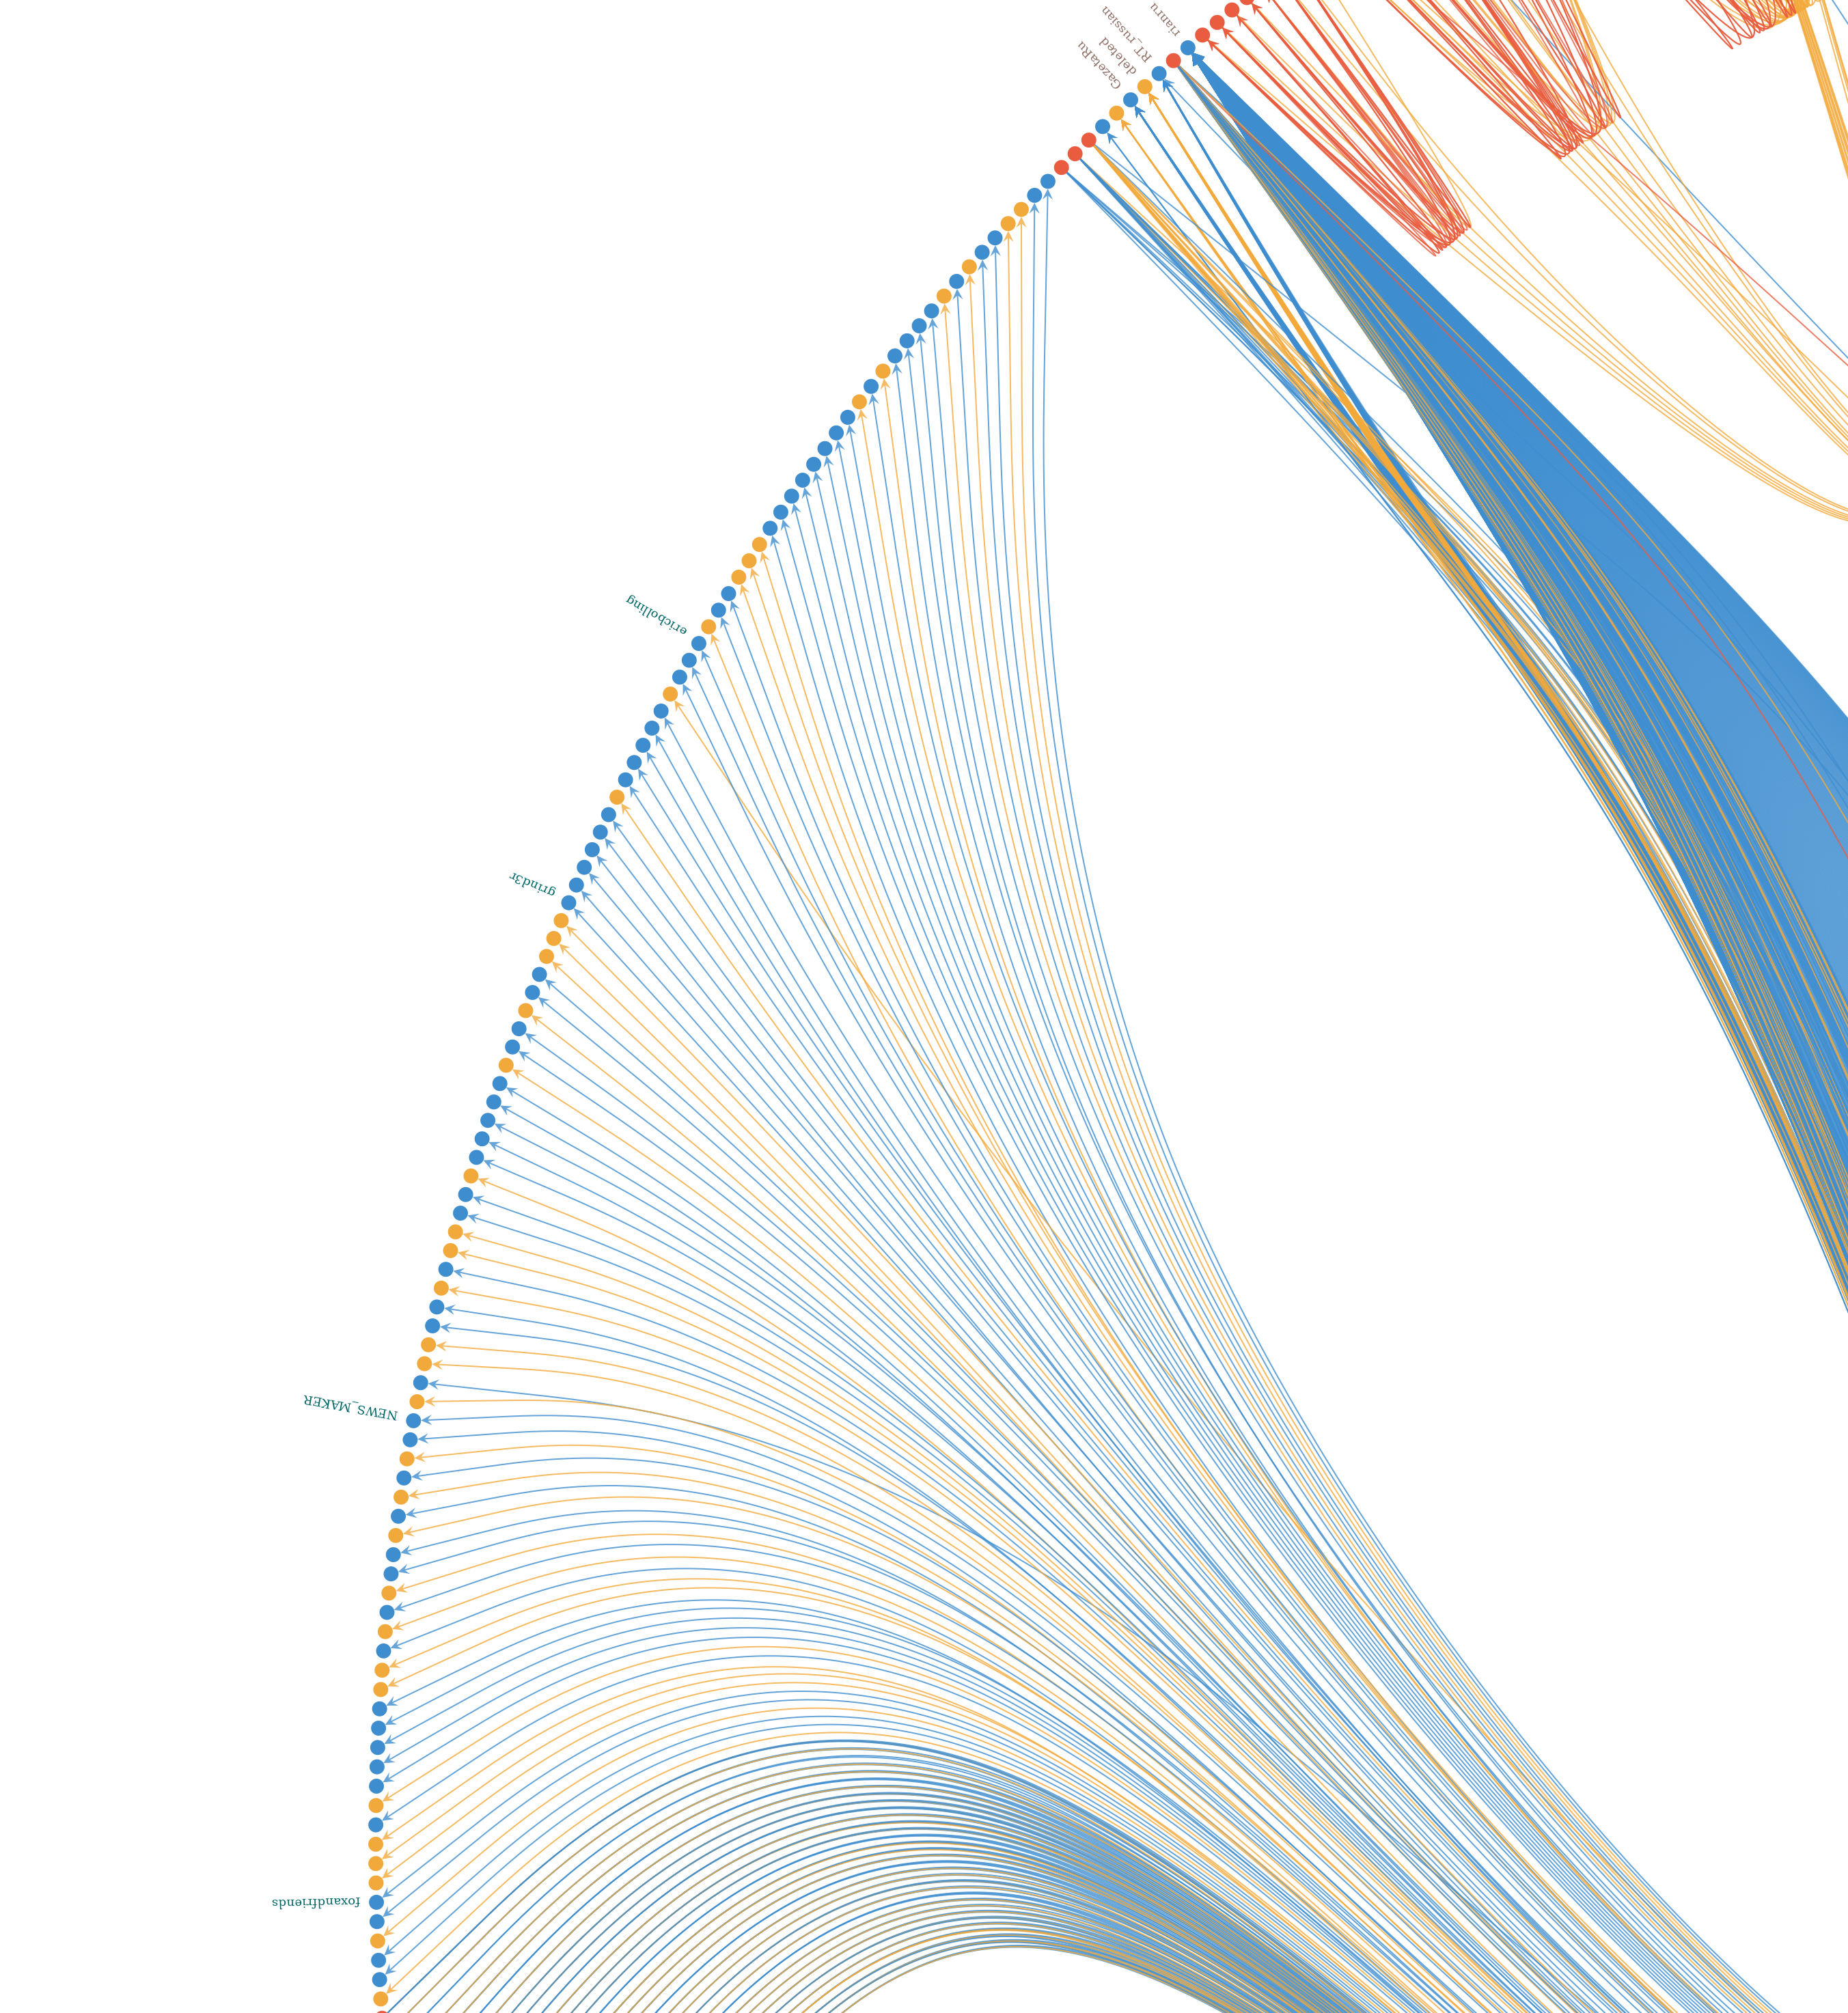
\includegraphics[width=0.4\textwidth,height=\textheight]{figures/Browne-Crick-McLevey-2023-Figure-8-Subplot-A.png}

\subcaption{\label{fig-ira1}}

\end{minipage}%
\newline
\begin{minipage}{\linewidth}

\captionsetup{labelsep=none}\includegraphics[width=0.4\textwidth,height=\textheight]{figures/Browne-Crick-McLevey-2023-Figure-8-Subplot-B.png}

\subcaption{\label{fig-ira2}}

\end{minipage}%
\newline
\begin{minipage}{\linewidth}

\captionsetup{labelsep=none}\includegraphics[width=0.4\textwidth,height=\textheight]{figures/Browne-Crick-McLevey-2023-Figure-8-Subplot-C.png}

\subcaption{\label{fig-ira3}}

\end{minipage}%

\caption{\label{fig-8}Three different enlarged views of the filtered IRA
Network.}

\end{figure}%

The network visualizations in Figure~\ref{fig-8} show an enlarged view
of some key distinct patterns in the network. Subplot A shows a small
number of IRA accounts targeting Twitter accounts of non-descript
origin, and primarily spreading conspiracy theories of the
time.\footnote{Such as Barack Obama being born in Kenya. More recently,
  these accounts post about Covid-19 conspiracies.} The second image
shows activity focused on popular US media organizations, like
\emph{Mashable}, \emph{The Washington Post}, and \emph{Fox News}. In the
third image is a mix, with \emph{Al Jazeera}, the \emph{Financial
Times}, and a popular Russia-based satire account as targets. There is a
great deal of in-depth analysis that could be undertaken here, but it
does seem evident that the activity of these accounts was not solely
focused on the US election, especially given the attention paid to
\emph{RIA Novosti} (\emph{rianru}).

Inference about the goals behind these Twitter strategies might be
possible, but not without care -- how would a foreign influence
objective be distinguishable from purposefully crafting the
\emph{impression} of foreign influence, for other purposes? And how
would the intended audience be identified? When 100 accounts send 10,000
Tweets each at the \emph{New York Times}, they are almost certainly not
banking on the producers of that newspaper to consider their statements.
In still other settings, it turns out that none of these considerations
even matter, where the reality is that bots are just tweeting amongst
each other (\citeproc{ref-thread2021bots}{Thread 2021}).

As the two foregoing analyses have made abundantly clear, BSBMs are
powerful tools for drawing inferences about the processes that give rise
to social structure in networks. What should be equally clear, however,
is that researchers must exercise caution when interpreting said
inferences. In our analysis of the Enron email network, we saw that
BSBMs admirably retrodict some of the structures we might expect to see
in a hierarchical network of corporate communications, but were equally
made aware of the fact that BSBMs do not necessarily measure any
particular kind of `ground truth' -- or if they do, that it may not be
the same ground truth researchers expect to draw inferences about. As H.
White, Boorman, and Breiger (\citeproc{ref-white1976social}{1976}),
Robins (\citeproc{ref-robins2011exponential}{2011}); and Nadel
(\citeproc{ref-nadel2013theory}{{[}1957{]} 2013}) are wont to emphasize:
social roles are complex, embedded, and multifaceted: researchers cannot
hope to apprehend the totality of a social role through the analysis of
one kind of social tie. In our analysis of the IRA disinformation
campaign on Twitter, we encountered the pitfalls of ascribing a causal
story to the patterns of behaviour hinted at by the results of a BSBM:
the same results can be easily re-interpreted to support conclusions
that emphasize the foreign influence role of IRA activity, the domestic
influence role of IRA activity, or the seemingly impotent bot-on-bot IRA
activity.

\section{Conclusion}\label{conclusion}

In this chapter, we introduced readers to the Bayesian Stochastic
Blockmodel -- which is a powerful inferential counterpart to prevailing
descriptive approaches to community detection and network clustering --
and demonstrated the process of applying and interpreting BSBMs in two
very different contexts. As with all unsupervised learning, great care
is required when specifying and drawing inferences from the graph
partitions we obtain by developing and fitting BSBMs. This is not
because SBMs are uniquely prone to misapplication or are otherwise
unwieldy. BSBMs open many exciting research opportunities for network
scientists by combining decades of insightful work on equivalence,
blockmodels, and network clustering (see Dorien, this volume) with
probabilistic thinking and generative modelling. But, as with all other
approaches, we need careful and deliberate analysis to make inferences
about meaningful human behaviour.

\section*{References}\label{references}
\addcontentsline{toc}{section}{References}

\phantomsection\label{refs}
\begin{CSLReferences}{1}{0}
\bibitem[\citeproctext]{ref-anderson1992building}
Anderson, Carolyn, Stanley Wasserman, and Katherine Faust. 1992.
{``Building Stochastic Blockmodels.''} \emph{Social Networks} 14 (1-2):
137--61.

\bibitem[\citeproctext]{ref-arabie1982blockmodels}
Arabie, Phipps, Scott A Boorman, et al. 1982. {``Blockmodels:
Developments and Prospects.''} In \emph{Classifying Social Data: New
Applications of Analytic Methods for Social Science Research}, edited by
Herschel C. Hudson, 177--98. Jossey-Bass San Francisco.

\bibitem[\citeproctext]{ref-arabie1978constructing}
Arabie, Phipps, Scott A Boorman, and Paul Levitt. 1978. {``Constructing
Blockmodels: How and Why.''} \emph{Journal of Mathematical Psychology}
17 (1): 21--63.

\bibitem[\citeproctext]{ref-aven2015paradox}
Aven, Brandy. 2015. {``The Paradox of Corrupt Networks: An Analysis of
Organizational Crime at Enron.''} \emph{Organization Science} 26 (4):
980--96.

\bibitem[\citeproctext]{ref-blondel2008fast}
Blondel, Vincent, Jean-Loup Guillaume, Renaud Lambiotte, and Etienne
Lefebvre. 2008. {``Fast Unfolding of Communities in Large Networks.''}
\emph{Journal of Statistical Mechanics: Theory and Experiment} 2008
(10): P10008.

\bibitem[\citeproctext]{ref-boorman1976social}
Boorman, Scott A, and Harrison White. 1976. {``Social Structure from
Multiple Networks. II. Role Structures.''} \emph{American Journal of
Sociology} 81 (6): 1384--1446.

\bibitem[\citeproctext]{ref-breiger1975algorithm}
Breiger, Ronald, Scott A Boorman, and Phipps Arabie. 1975. {``An
Algorithm for Clustering Relational Data with Applications to Social
Network Analysis and Comparison with Multidimensional Scaling.''}
\emph{Journal of Mathematical Psychology} 12 (3): 328--83.

\bibitem[\citeproctext]{ref-clayton2021bernoulli}
Clayton, Aubrey. 2021. \emph{Bernoulli's Fallacy: Statistical Illogic
and the Crisis of Modern Science}. New York: Columbia University Press.

\bibitem[\citeproctext]{ref-collins1988theoretical}
Collins, Randall. 1988. \emph{Theoretical Sociology}. San Francisco:
Harcourt Brace Jovanovich.

\bibitem[\citeproctext]{ref-corneli2019dynamic}
Corneli, Marco, Charles Bouveyron, Pierre Latouche, and Fabrice Rossi.
2019. {``The Dynamic Stochastic Topic Block Model for Dynamic Networks
with Textual Edges.''} \emph{Statistics and Computing} 29: 677--95.

\bibitem[\citeproctext]{ref-cox1946probability}
Cox, Richard. 1946. {``Probability, Frequency and Reasonable
Expectation.''} \emph{American Journal of Physics} 14 (1): 1--13.

\bibitem[\citeproctext]{ref-diesner2005exploration}
Diesner, Jana, and Kathleen Carley. 2005. {``Exploration of
Communication Networks from the Enron Email Corpus.''} In \emph{SIAM
International Conference on Data Mining: Workshop on Link Analysis,
Counterterrorism and Security, Newport Beach, CA}, 3--14.

\bibitem[\citeproctext]{ref-dorien2023shsna3bpr}
Dorien, Patrick, Anuška Ferligoj, and Vladimir Batagelj. 2024.
{``Blockmodelling, Positions, and Roles.''} In \emph{The SAGE Handbook
of Social Network Analysis (Volume 2)}, edited by John McLevey, John
Scott, and Peter J Carrington, 404--16. London: SAGE.

\bibitem[\citeproctext]{ref-Erdos1959pmd}
Erdös, P, and A Rényi. 1959. {``On Random Graphs i.''}
\emph{Publicationes Mathematicae Debrecen} 6: 290--97.

\bibitem[\citeproctext]{ref-erickson1988relational}
Erickson, Bonnie. 1988. {``The Relational Basis of Attitudes.''} In
\emph{Social Structures: A Network Approach}, edited by Barry Wellman
and Stephen Berkowitz. Cambridge: Cambridge University Press.

\bibitem[\citeproctext]{ref-festinger1949analysis}
Festinger, Leon. 1949. {``The Analysis of Sociograms Using Matrix
Algebra.''} \emph{Human Relations} 2 (2): 153--58.

\bibitem[\citeproctext]{ref-friedkin1984structural}
Friedkin, Noah. 1984. {``Structural Cohesion and Equivalence
Explanations of Social Homogeneity.''} \emph{Sociological Methods \&
Research} 12 (3): 235--61.

\bibitem[\citeproctext]{ref-grace2022disinfo}
Grace, Perri. 2022. {``Inside Russia's Domestic Disinformation
Ecosystem.''} Inkstick.
\url{https://inkstickmedia.com/inside-russias-domestic-disinformation-ecosystem/}.

\bibitem[\citeproctext]{ref-grunwald2007minimum}
Grünwald, Peter D. 2007. \emph{The Minimum Description Length
Principle}. MIT press.

\bibitem[\citeproctext]{ref-hardin2015network}
Hardin, JS, Ghassan Sarkis, and PC Urc. 2015. {``Network Analysis with
the Enron Email Corpus.''} \emph{Journal of Statistics Education} 23
(2).

\bibitem[\citeproctext]{ref-holland1983stochastic}
Holland, Paul, Kathryn Blackmond Laskey, and Samuel Leinhardt. 1983.
{``Stochastic Blockmodels: First Steps.''} \emph{Social Networks} 5 (2):
109--37.

\bibitem[\citeproctext]{ref-jaynes2003probability}
Jaynes, Edwin. 2003. \emph{Probability Theory: The Logic of Science}.
Cambridge: Cambridge University Press.

\bibitem[\citeproctext]{ref-klimt2004introducing}
Klimt, Bryan, and Yiming Yang. 2004. {``Introducing the Enron Corpus.''}
In \emph{CEAS}, 45:92--96.

\bibitem[\citeproctext]{ref-leskovec2009community}
Leskovec, Jure, Kevin Lang, Anirban Dasgupta, and Michael Mahoney. 2009.
{``Community Structure in Large Networks: Natural Cluster Sizes and the
Absence of Large Well-Defined Clusters.''} \emph{Internet Mathematics} 6
(1): 29--123.

\bibitem[\citeproctext]{ref-light1979primer}
Light, John, and Nicholas Mullins. 1979. {``A Primer on Blockmodeling
Procedure.''} In \emph{Perspectives on Social Network Research}, edited
by Paul Holland and Samuel Leinhardt, 85--118. New York: Academic Press.

\bibitem[\citeproctext]{ref-lorrain1971structural}
Lorrain, Francois, and Harrison White. 1971. {``Structural Equivalence
of Individuals in Social Networks.''} \emph{The Journal of Mathematical
Sociology} 1 (1): 49--80.

\bibitem[\citeproctext]{ref-luce1949method}
Luce, Duncan, and Albert Perry. 1949. {``A Method of Matrix Analysis of
Group Structure.''} \emph{Psychometrika} 14 (2): 95--116.

\bibitem[\citeproctext]{ref-matsuyama2008analyzing}
Matsuyama, Shinako, and Takao Terano. 2008. {``Analyzing the ENRON
Communication Network Using Agent-Based Simulation.''} \emph{Journal of
Networks} 3 (7): 26--33.

\bibitem[\citeproctext]{ref-mcelreath2020statistical}
McElreath, Richard. 2020. \emph{Statistical Rethinking: A Bayesian
Course with Examples in {R} and STAN}. New York: Chapman; Hall/CRC.

\bibitem[\citeproctext]{ref-moody2023shsna2cohesion}
Moody, James, and Peter J Mucha. 2024. {``Structural Cohesion and
Cohesive Subgroups.''} In \emph{The SAGE Handbook of Social Network
Analysis (Volume 2)}, edited by John McLevey, John Scott, and Peter J
Carrington, 376--91. London: SAGE.

\bibitem[\citeproctext]{ref-nadel2013theory}
Nadel, Siegfried Frederick. (1957) 2013. \emph{The Theory of Social
Structure}. Vol. 8. Routledge.

\bibitem[\citeproctext]{ref-newman2020improved}
Newman, Mark, George Cantwell, and Jean-Gabriel Young. 2020. {``Improved
Mutual Information Measure for Clustering, Classification, and Community
Detection.''} \emph{Physical Review E} 101 (4): 042304.

\bibitem[\citeproctext]{ref-nowicki2001estimation}
Nowicki, Krzysztof, and Tom AB Snijders. 2001. {``Estimation and
Prediction for Stochastic Blockstructures.''} \emph{Journal of the
American Statistical Association} 96 (455): 1077--87.

\bibitem[\citeproctext]{ref-peixoto2014efficient}
Peixoto, Tiago. 2014a. {``Efficient Monte Carlo and Greedy Heuristic for
the Inference of Stochastic Block Models.''} \emph{Physical Review E} 89
(1): 012804.

\bibitem[\citeproctext]{ref-peixoto2014graph}
---------. 2014b. {``The Graph-Tool Python Library.''} \emph{Figshare}.
\url{https://doi.org/10.6084/m9.figshare.1164194}.

\bibitem[\citeproctext]{ref-peixoto2019bayesian}
---------. 2019. {``Bayesian Stochastic Blockmodeling.''} In
\emph{Advances in Network Clustering and Blockmodeling}, edited by
Patrick Doreian, Vladimir Batagelj, and Anuska Ferligoj, 289--332.
Oxford: John Wiley \& Sons.

\bibitem[\citeproctext]{ref-peixoto2021revealing}
---------. 2021. {``Revealing Consensus and Dissensus Between Network
Partitions.''} \emph{Physical Review X} 11 (2): 021003.

\bibitem[\citeproctext]{ref-peixoto2023descriptive}
---------. 2023. {``Descriptive Vs. Inferential Community Detection in
Networks: Pitfalls, Myths and Half-Truths.''} \emph{Elements in the
Structure and Dynamics of Complex Networks}.

\bibitem[\citeproctext]{ref-robins2011exponential}
Robins, Garry. 2011. {``Exponential Random Graph Models for Social
Networks.''} In \emph{The SAGE Handbook of Social Network Analysis},
edited by John Scott and Peter J Carrington, 484--500. London: Sage.

\bibitem[\citeproctext]{ref-roeder3we}
Roeder, Oliver. n.d. {``We Gave You 3 Million Russian Troll Tweets.
Here's What You've Found so Far, 2018.''} FiveThirtyEight.
\url{https://fivethirtyeight.com/features/what-we-found-in-3-million-russian-troll-tweets/}.

\bibitem[\citeproctext]{ref-ruhe2016enron}
Ruhe, Arne Hendrik. 2016. {``Enron Data.''}
www.ahschulz.de/enron-email-data/.

\bibitem[\citeproctext]{ref-mclevey2023shsna1intro}
Scott, John, John McLevey, and Peter J Carrington. 2024.
{``Introduction.''} In \emph{The SAGE Handbook of Social Network
Analysis (Volume 2)}, edited by John McLevey, John Scott, and Peter J
Carrington, 1--18. London: SAGE.

\bibitem[\citeproctext]{ref-shannon1948mathematical}
Shannon, Claude. 1948. {``A Mathematical Theory of Communication.''}
\emph{The Bell System Technical Journal} 27 (3): 379--423.

\bibitem[\citeproctext]{ref-snijders1997estimation}
Snijders, Tom AB, and Krzysztof Nowicki. 1997. {``Estimation and
Prediction for Stochastic Blockmodels for Graphs with Latent Block
Structure.''} \emph{Journal of Classification} 14 (1): 75--100.

\bibitem[\citeproctext]{ref-somerville2020disinformation}
Somerville, Alistair, and Jonas Heerin. 2020. {``The Disinformation
Shift: From Foreign to Domestic.''} \emph{Georgetown Journal of
International Affairs}.

\bibitem[\citeproctext]{ref-thread2021bots}
Thread, Common. 2021. {``Four Truths about Bots.''} Twitter.
\url{https://blog.twitter.com/common-thread/en/topics/stories/2021/four-truths-about-bots}.

\bibitem[\citeproctext]{ref-traag2019louvain}
Traag, Vincent, Ludo Waltman, and Nees Jan Van Eck. 2019. {``From
Louvain to Leiden: Guaranteeing Well-Connected Communities.''}
\emph{Scientific Reports} 9 (1): 5233.

\bibitem[\citeproctext]{ref-vanburen2009enron}
VanBuren, Victoria, David Villarreal, Thomas McMillen, and Andrew
Minnicks. 2009. {``Enron Dataset Research: E-Mail Relevance
Classification.''}

\bibitem[\citeproctext]{ref-wang1987stochastic}
Wang, Yuchung, and George Wong. 1987. {``Stochastic Blockmodels for
Directed Graphs.''} \emph{Journal of the American Statistical
Association} 82 (397): 8--19.

\bibitem[\citeproctext]{ref-wasserman1987stochastic}
Wasserman, Stanley, and Carolyn Anderson. 1987. {``Stochastic a
Posteriori Blockmodels: Construction and Assessment.''} \emph{Social
Networks} 9 (1): 1--36.

\bibitem[\citeproctext]{ref-stanley1994social}
Wasserman, Stanley, and Katherine Faust. 1994. \emph{Social Network
Analysis: Methods and Applications}. Cambridge: Cambridge University
Press.

\bibitem[\citeproctext]{ref-white1983graph}
White, Douglas, and Karl Reitz. 1983. {``Graph and Semigroup
Homomorphisms on Networks of Relations.''} \emph{Social Networks} 5 (2):
193--234.

\bibitem[\citeproctext]{ref-white1976social}
White, Harrison, Scott A Boorman, and Ronald Breiger. 1976. {``Social
Structure from Multiple Networks. I. Blockmodels of Roles and
Positions.''} \emph{American Journal of Sociology} 81 (4): 730--80.

\bibitem[\citeproctext]{ref-wilson2009discovery}
Wilson, Garnett, and Wolfgang Banzhaf. 2009. {``Discovery of Email
Communication Networks from the Enron Corpus with a Genetic Algorithm
Using Social Network Analysis.''} In \emph{2009 IEEE Congress on
Evolutionary Computation}, 3256--63. IEEE.

\bibitem[\citeproctext]{ref-zhang2020statistical}
Zhang, Lizhi, and Tiago Peixoto. 2020. {``Statistical Inference of
Assortative Community Structures.''} \emph{Physical Review Research} 2
(4): 043271.

\bibitem[\citeproctext]{ref-zondervan2017priors}
Zondervan-Zwijnenburg, Mariëlle, Margot Peeters, Sarah Depaoli, and Rens
Van de Schoot. 2017. {``Where Do Priors Come from? Applying Guidelines
to Construct Informative Priors in Small Sample Research.''}
\emph{Research in Human Development} 14 (4): 305--20.

\end{CSLReferences}



\end{document}
